\section{Gaussian Multi User Channels}
From the previous sections of the paper , the output of a Gaussian Channel with input power \( P \) and noise variance \( N \) is given by:
\begin{equation}
Y_i = X_i + Z_i, \quad i = 1, 2, \ldots
\end{equation}
In the above equation, There is a power constraint on signal \( X = (X_1, X_2, \ldots, X_n) \) 
\begin{equation}
\frac{1}{n} \sum_{i=1}^n X_i^2 \leq P.
\end{equation}
 and \( Z_i \) are i.i.d. Gaussian RV's with mean 0 and variance \( N \). 
The capacity of Gaussian Channel is given by:
\begin{equation}
C = \frac{1}{2} \log \left( 1 + \frac{P}{N} \right) \text{ bits per transmission.}
\end{equation}

Below , are different types of discrete-time memoryless Gaussian channels.

\subsection{Single User Gaussian Channel}
Choosing an index \( i \) in the set \( 2^{nR} \) in a codebook \( (2^{nR}, n) \) with rate \( R < \frac{1}{2} \log(1 + \frac{P}{N}) \). \( Y = X(i) + Z \) is observed by the receiver, and from \( Y \), receiver tries to find the index \( i \).
Probability of error \( P_e\) will be arbitrarily small when \( n \) is sufficiently large.For finding the codeword in the codebook that is jointly typical with the received vector \( Y \),this minimum distance decoding scheme is essential.

\subsection{Gaussian Multiple Access Channel with \( m \) Users} \label{sec 6.2}
The observed output with \( m \) transmitters is:
\begin{equation}
Y = \sum_{i=1}^m X_i + Z.
\end{equation}
Considering the signal-to-noise ratio \( P/N \) of a single user Gaussian channel, the capacity and rate are related as:
\begin{equation}
C \left( \frac{P}{N} \right) = \frac{1}{2} \log \left( 1 + \frac{P}{N} \right)
\end{equation}
\begin{equation}
R_i < C \left( \frac{P}{N} \right)
\end{equation}
Taking $2$ users in a similar way, 
\begin{equation}
R_i + R_j < C \left( \frac{2P}{N} \right).
\end{equation}
Taking $3$ users in a similar way, 
\begin{equation}
R_i + R_j + R_k < C \left( \frac{3P}{N} \right).
\end{equation}
Extending the above to $m$ users,
\begin{equation}
\vdots
\end{equation}
\begin{equation}
\sum_{i=1}^m R_i < C \left( \frac{mP}{N} \right).
\end{equation}
Gaussian Channel with \( m \) users can be understood in lines of a single user with a slight difference that there are \( 2^{n R_i} \) codewords within an \( i \)th codebook and there are  \( m \) codebooks 
An arbitrary codeword is chosen by each independent transmitter from its own codebook. 
\\All vectors are simultaneously sent by the user, and hence, each transmitter uses the entire bandwidth at all times. All the codewords when added with Gaussian noise \( Z \) is observed by the receiver.
When it comes to decoding, optimality is achieved when looking for each codebook, where \( m \) codewords such that the vector sum is closest to \( Y \).
In the capacity region shown above from \( R1 \) to \( R_m \) ,then \( P_e\) goes to $0$ as \( n \) tends to $\infty$.

\subsection{Gaussian Broadcast Channel}
In this type of channel, there are $2$ receivers that are distinct in terms of noise power $ie$ having \( N_1 \) and \( N_2 \) with the same signal power  \( P \). Assuming \( N_1 < N_2 \), then it implies that there is less noise in the receiver $Y1$ when compared to $Y2$, the output of each Gaussian Channel is given by the same formula,
\begin{equation}
Y_1 = X + Z_1  
\end{equation}
\begin{equation}
Y_2 = X + Z_2  
\end{equation}
in the above, it is to note that sender wants to send messages to receivers \( Y_1 \) and \( Y_2 \) at rates \( R_1 \) and \( R_2 \) and that  \( Z_1 \) is a correlated Gaussian RVs with $\mathrm{Var}$ \( N_1 \) and similarly  \( Z_1 \) with $\mathrm{Var}$ \( N_2 \).
The Channel Capacity and Rate of a Gaussian Broadcast Channel are related as:
For Rate $R1$,
\begin{equation}
R_1 < C \left( \frac{\alpha P}{N_1} \right).
\end{equation}
For Rate $R2$,
\begin{equation}
R_2 < C \left( \frac{(1 - \alpha)P}{\alpha P + N_2} \right),
\end{equation}
where \( (0 \leq \alpha \leq 1) \) is chosen by the transmitter.
\\
The transmitter takes the codeword \( X(i) \) where \( i \in \{1, 2, \ldots, 2^{n R_1}\} \) to send to \( Y_1 \) and \( X(j) \) where \( j \in \{1, 2, \ldots, 2^{n R_2}\} \) to send to \( Y_2 \), combines the sum and sent it over the Channel.
\\
Decoding is to be done at the receiver, recalling the assumption made before \( N_1 < N_2 \), bad receiver \( Y_2 \) is considered first and by looking through to find the closest codeword, the effective  \( P/N \) is seen as \( \frac{\beta P}{\alpha P + N_2} \) since the noise to $Y2$ is the message $Y1$.
After which, the good receiver \( Y_1 \) decodes codeword of \( Y_2 \), which can be easily due to the assumption that $N1$ has lower noise.Now \( X(j) \) codeword is subtracted from $Y1$, then the search for codeword closest to \( Y_1 - X(j) \) begins, and \( P_e\) is low.
\\
Similarly, for Optimal Encoding, the above method is quite efficient since receiver $Y1$ is aware of the message intended for it as well as $Y2$.

\subsection{Gaussian Relay Channel}
In this type of Gaussian Channel, there is a sender $X$ and receiver \( Y \) along with a Relay Channel to help the receiver, the output of the channel is described as :
\begin{equation}
Y_1 = X + Z_1,
\end{equation}
\begin{equation}
Y = X + Z_1 + X_1 + Z_2,
\end{equation}

Encoding by the relay, which is allowed, is 
\begin{equation}
X_1 = f(Y_1, Y_{12}, \ldots, Y_{1, t-1}).
\end{equation} 
and \( Z_1 \) is a independent Gaussian RVs with $\mathrm{Var}$ \( N_1 \) and
$\mu$ as $0$ similarly  \( Z_1 \) with $\mathrm{Var}$ \( N_2 \)  and $\mu$ as $0$.
If the power is $P1$ of sender $X1$ and $P$ of $X$, the capacity is given by:
\begin{equation}
C = \max_{0 \leq \alpha \leq 1} \min \left( \frac{P + P_1 + 2\sqrt{\bar{\alpha} P P_1}}{N_1 + N_2}, C(\frac{ \alpha P}{N_1}) \right)
\end{equation}
where \( \bar{\alpha} = 1 - \alpha \) and when 
\begin{equation}
\frac{P1}{N_2} \ge \frac{P}{N_1}, \tag{3}
\end{equation}
and  \( \alpha = 1 \) , $C$ becomes \( C(P/N_1) \) $ie$ the channel after the Relay appears to be noise free and from $X$ , \( C(P/N_1) \) is possible and in the case where is no Relay the rate \( C(P/(N_1 + N_2)) \) gets increased due to presence of signal power $P$ and noise $N1$.
When $N2$ is also large enough and the $eq $ $3$ gets statisfied , then rate increases from \( C(P/(N_1 + N_2)) \) to \( C(P/N_1) \).
\\
Two codebooks will be needed if \( R_1 < C(\alpha P/N_1) \). $1st$ codebook has power \( \alpha P \) with  \( 2^{nR_1} \) words , similarly $2nd$ has \( \bar{\alpha} P \) power and \( 2^{nR_0} \) codewords.After sending the codeword from the $1st$ codebook, since \( R_1 < C(\alpha P/N_1) \), index of the codeword is known by the relay, and all possible codewords list is available with the receiver of size 
\( 2^{n(R_1 - C(\alpha P/(N_1 + N_2)))} \). 
There is an uncertainty with the codeword on the receiver's list since it is unaware of the received signal \( Y \).
\\Then , by randomly partitioning and getting \( 2^{nR_0} \) cells from $1st$ codebook such that equal codewords exist in each of the \( 2^{nR_0} \) cells, after which search for the cell in which $1st$ codeword lies and after finding it , it is sent to the $2nd $ codeword with the same index, that is how \( X \) and \( X_r \) are sent the same codeword and the relay now must scale this codeword such that the power constraint \( P_r \) is met.
\\After which both \( X \) and \( X_r \) trasmit the codewords , information is sent coherently by both the transmitter and receiver hence the power observed by \( Y \) is \( (\sqrt{\alpha P} + \sqrt{P_r})^2 \).
\newpage
Another codeword from $1st$ codebook is chosen by the transmitter in the $2nd $ block, and after adding it to the $2nd $ codebook , it is sent over the channel.The receiver \( Y \) looks for the closest codeword in $2nd$ codebook and it is subtracted from the received sequence, hence the  capacity is indices of size \(2^{N_0}\).
Receiver \( Y \) intersects the list from possible codeword in $1st$ block to the ones in relay transmission of $2nd$ block to complete the computing of codeword from $1st$ codebook and \(Y\)'s guess is sent to $1st$ block. Power and Rate has to be chosen carefully such that there is only $1$ codeword in the receiver \( Y \) intersection.
\\
After reaching steady state , transmitter and relay resolve the list uncertainity as mentioned in the above step and each time the former adds information from $1st$ codebook to the $2nd$ and the sum is transmitted , which make the receiver $1$ block behind but it is to also note that this delay does not affect rate of reception overall.

\subsection{Gaussian Interference Channel}
This type of channel is quite different from the ones discussed above as it is has $2$ senders and receivers and also sender $1$ sends information only to receiver $1$ and doesnot care about the other receiver understanding, similarly with sender $2$ and receiver $2$.The outputs of this channel can be described as :
\begin{equation}
    Y_1 = X_1 + aX_2 + Z_1
\end{equation}
\begin{equation}
    Y_2 = X_2 + aX_1 + Z_2,
\end{equation}
\( Z_1 \) is a independent Gaussian RVs with $\mathrm{Var}$ \( N_1 \) and
$\mu$ as $0$ similarly  \( Z_1 \) with $\mathrm{Var}$ \( N_2 \)  and $\mu$ as $0$.
\begin{center}
	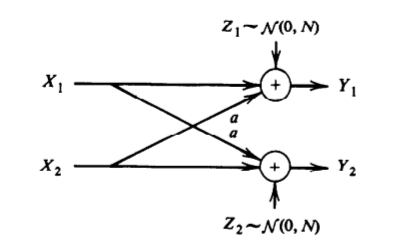
\includegraphics[scale=0.5]{Diagrams/Gaussian_Interference_Channel.png}
\end{center} 
For the above channel , there needs to be $2$ codebooks generated each with a power $P$ and with rate \( C(P/N) \).If the interference is \( a^2 P/(P + N) > C(P/N) \), index of the $2nd$ transmitter is understood by the $1st$ by looking for the closest word in the signal that is received and after the signal is found , it is subtracted from its signal to have a clean channel between this and sender.After that is done , now the sender's codewords are searched for the closest codeword and then it is declared as the one which is sent.

\subsection{Gaussian Two-Way Channel}
This Channel is similar to the one discussed above but with a change that Gaussian Two-Way channel has Feedback and here senders of both are attached to the other receiver $ie$ upon understanding the previous received symbols of receiver $2$ , sender $1$ can decide what can be sent next.
\begin{center}
	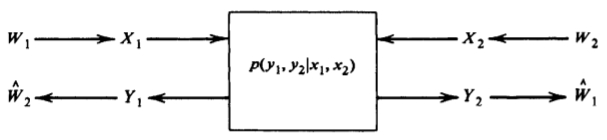
\includegraphics[scale=0.5]{Diagrams/Gaussian_Two-Way_Channel.png}
\end{center} 
For transmitters $1$ and $2$ if the power and noise $\mathrm{Var}$ are  \( P_1 \) ,\( P_2 \) ;\( N_1 \), \( N_2 \);Rates are given by:
\begin{equation}
    R_1 < C(P_1/N_1) 
\end{equation}
\begin{equation}
    R_2 < C(P_2/N_2)
\end{equation}
The Channel can be acheived by generating $2$ codebooks $R1$ and $R2$ and after the codeword from codebook is sent by senders , the sum of codewords along with some noise is received by receiver $2$ , then the codeword from sender $2$ is subtracted to get a clean channel from sender $1$ which also has some noise $N1$ as discussed above. Two-Way Gaussian channel can be viewed through the lens of $2$ independent Gaussian Channels , but there is a slight trade off with such channels which both cannot send information in the most optimal way at the same time.